\newpage\EMPHASIZE{22. Reference Parameters}

\textsc{Objectives}
\begin{itemize}
\item Understand and use reference variables
\item Write functions with reference parameters
\end{itemize}

You have already seen references (or reference variables). This chapter is a quick review and some more information on references.


\newpage\EMPHASIZE{Problems with Our Functions}

What about writing a function to perform ``array assignment'', i.e., we want to do the following:

\begin{consolethree}[escapeinside=||]
int x[] = {1,2,3};
int xSize = 3;
int y[3];
int ySize = 3;
arrayAssign(y, 3, x, 3); // like y = x
\end{consolethree}

That's easy: Just write a for-loop in the function to pass the values from one to the other.

This works for arrays of the same size. What if I use a ``length'' for an array?

What I mean is that suppose I have an array of size 1000. I want to use the array like a container: I want to put values into the array and I want to pull values out of the array. The length of an array measures the number of things I put into the array that has not been taken out. For instance suppose I have the following:

\begin{consolethree}[escapeinside=||]
const int GOOGLE_STOCK_PRICE_SIZE = 1000;
double googleStockPrice[GOOGLE_STOCK_PRICE_SIZE];
\end{consolethree}

which records the stock as the day progresses. \texttt{googleStockPrice[0]} is the stock price of Google at 9:00AM when the stock market opens, and \texttt{googleStockPrice[1]} is the stock price at 9:01AM, etc. At 9:05AM, I have stock prices of Google for 9:00AM, 9:01AM, 9:02AM, 9:03AM, 9:04AM, 9:05AM, i.e. there are 6 values. Of course the array has a size of 1000. But only \texttt{googleStockPrice[i]} for i = 0, 1, 2, 3, 4, 5 are valid at that point in time. I can keep track of how many values (from index 0) are valid using an integer variable, say \texttt{googleStockPriceLen} (Len for length).

\begin{consolethree}[escapeinside=||]
const int GOOGLE_STOCK_PRICE_SIZE = 1000;
double googleStockPrice[GOOGLE_STOCK_PRICE_SIZE];
int googleStockPriceLen = 0;
\end{consolethree}

So make sure you see the difference between the two different measures of an array: one measures the \EMPHASIZE{total number of values the array can hold}, and the other measures \EMPHASIZE{the number of values that have been placed into the array that has not been taken out}.

Now suppose we want to write an array assignment function for such a general situation (remember: you want functions to be re-usable, therefore you want to make them general enough), then you want to be able to do this:

\begin{consolethree}[escapeinside=||]
const int XSIZE = 10;
int x[XSIZE] = {42, 41, 40};
int xlen = 3;
const int YSIZE = 10;
int y[YSIZE];
int ylen = 0;
arrayAssign(y, ylen, x, xlen); // sorta like y = x
\end{consolethree}

After the function call you want \texttt{y[0] = 42}, \texttt{y[1] =
41}, \texttt{y[2] = 40} and \texttt{ylen = 3.}

Now note this: A function can change the values of \texttt{y} which is an array. But the problem is that \texttt{ylen} is an integer variable and hence cannot be changed by a function when it is passed in as a pass-by-value parameter. Right? Here's an example:

\begin{consolethree}[escapeinside=||]
void swap(int a, int b)
{
    int t = a;
    a = b;
    b = t;
}

int main()
{
    int x = 0;
    int y = 42;
    swap(x, y); // x, y NOT CHANGED!!!!!!!!!!!!!!!!!!
    std::cout << x << ' ' << y << std::endl;
    return 0;
}
\end{consolethree}

One way to get around that is that you can return a value from a function and use that to change the value of \texttt{ylen} in the calling function. So the code using the array assignment function would look like this:

\begin{consolethree}[escapeinside=||]
const int XSIZE = 10;
int x[XSIZE] = {42, 41, 40};
int xlen = 3;
const int YSIZE = 10;
int y[YSIZE];
int ylen = 0;
ylen = arrayAssign(y, x, xlen); // sorta like y = x
\end{consolethree}

That will work. \EMPHASIZE{But} the prototype of this function would look very different from other useful array functions. This is how a header file for all the useful array functions if you have one:

\begin{consolethree}[escapeinside=||]
// array.h
bool arrayEqual(int[], int, int[], int);
bool arrayNotEqual(int[], int, int[], int);
void bubbleSort(int[], int);
int binarySearch(int[], int, int target);
int arrayAssign(int[], int[], int);
\end{consolethree}

One quality of a well-designed program is one with \EMPHASIZE{least surprises}. In all parameters, you always see an array followed by a length ... EXCEPT for the case of \texttt{arrayAssign()}.

There's another problem with using return values to change variables: If you want to change the value of two variables through one single function call you CAN'T. \EMPHASIZE{A function cannot return two values at the same time}. The following \EMPHASIZE{does NOT work}:

\begin{consolethree}[escapeinside=||]
int,int swap(int a, int b)
{
    int t = a;
    a = b;
    b = t;
    return a, b // abominable
}

int main()
{
    int x = 0;
    int y = 42;
    x, y = swap(x, y); // :o
    return 0;
}
\end{consolethree}


\newpage\EMPHASIZE{Pass-by-Reference}

Now try this

\begin{consolethree}[escapeinside=||]
void swap(int & a, int & b)
{
    int t = a;
    a = b;
    b = t;
}

int main()
{
    int x = 0;
    int y = 42;
    swap(x, y);
    std::cout << x << ' ' << y << std::endl;
    return 0;
}
\end{consolethree}

The variables \texttt{a} and \texttt{b} are called \EMPHASIZE{reference variable}, in particular they are integer reference variables. They are different from the regular plain-jane variables. They \EMPHASIZE{do not have their own memory for keeping values}. They \textbf{refer} to other variables. A reference variable is an \EMPHASIZE{alias} of another variable.
\newpage
Now back to our program with the \texttt{swap()} function:

\begin{consolethree}[escapeinside=||]
void swap(int & a, int & b)
{
    int t = a;
    a = b;
    b = t;
}

int main()
{
    int x = 0;
    int y = 42;
    swap(x, y);
    std::cout << x << ' ' << y << std::endl;
    return 0;
}
\end{consolethree}
\sidenote
{
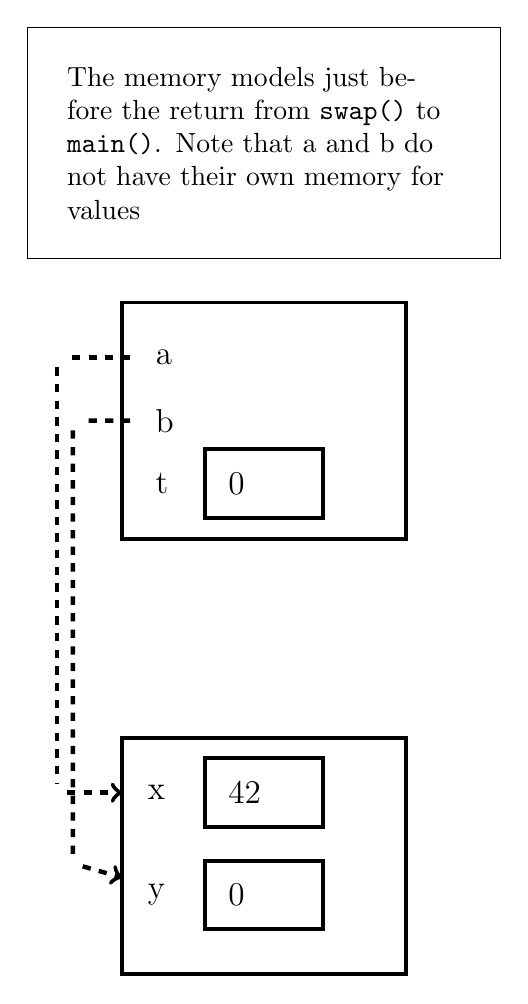
\begin{tikzpicture}
    \node[draw,text width=3cm,minimum height=3cm,minimum width=2cm, line width=0.05cm, inner sep=0.3cm] (a) at (-4,-2) {};
    \node[draw,text width=3cm,minimum height=3cm,minimum width=2cm, line width=0.05cm, inner sep=0.3cm, yshift=-4cm] (b) at (a.south) {};
    \node[xshift=-8mm, yshift=8mm] (a_arr) at (a.west) {};
    \node[xshift=-8mm, yshift=8mm] (a0_arr) at (b.west) {};
    \node[xshift=-6mm] (b_arr) at (a.west) {};
    \node[xshift=-6mm, yshift=-1mm] (b0_arr) at (b.west) {};
    \node[xshift=-6mm, yshift=-8mm] (c_arr) at (a.west) {};
    \node[xshift=-6mm, yshift=-8mm] (c0_arr) at (b.west) {};

    \node[text width=1mm,minimum height=1mm,minimum width=1mm, line width=0.05cm, inner sep=0.3cm, xshift=5mm, yshift=8mm] (aval) at (a.west) {\large{a}};
    \node[text width=1mm,minimum height=1mm,minimum width=1mm, line width=0.05cm, inner sep=0.3cm, xshift=5mm] (bval) at (a.west) {\large{b}};

    \node[text width=1mm,minimum height=1mm,minimum width=1mm, line width=0.05cm, inner sep=0.3cm, xshift=5mm, yshift=-8mm] (tval) at (a.west) {\large{t}};
    \node[draw, text width=9mm,minimum height=1mm,minimum width=5mm, line width=0.05cm, inner sep=0.3cm, yshift=-8mm] (tvalbox) at (a.center) {\large{0}};

    \node[text width=9mm,minimum height=1mm,minimum width=1mm, line width=0.05cm, inner sep=0.3cm, xshift=8mm, yshift=8mm] (xval) at (b.west) {\large{x}};
    \node[draw, text width=9mm,minimum height=1mm,minimum width=5mm, line width=0.05cm, inner sep=0.3cm, yshift=8mm] (xvalbox) at (b.center) {\large{42}};

    \node[text width=9mm,minimum height=1mm,minimum width=5mm, line width=0.05cm, inner sep=0.3cm, xshift=8mm, yshift=-5mm] (yval) at (b.west) {\large{y}};
    \node[draw, text width=9mm,minimum height=1mm,minimum width=5mm, line width=0.05cm, inner sep=0.3cm, yshift=-5mm] (yvalbox) at (b.center) {\large{0}};

    \draw [dashed, ultra thick, ->] (aval) -- (a_arr) -- (a0_arr) -- (xval);
    \draw [dashed, ultra thick, ->] (bval) -- (b_arr) -- (b0_arr) -- (yval)[xshift=-5mm];
    %this really doesnt look as good as i want it to, definitely needs another go after all other notes are finished
    \node[draw, text width=5cm,minimum height=2cm,minimum width=5cm, line width=0.0mm, inner sep=0.5cm, yshift=2cm] (text0) at (a.north) {\normalsize{The memory models just before the return from \texttt{swap()} to \texttt{main()}. Note that a and b do not have their own memory for values}};

\end{tikzpicture}
}

when \texttt{main()} calls \texttt{swap()}, the integer reference variable \texttt{a} in \texttt{swap()} will \EMPHASIZE{refer} to the memory of \texttt{x}; it \EMPHASIZE{does not receive a value} from \texttt{x}. As a matter of fact, referring the diagram, you see that \texttt{a} does not even have its own memory!

Likewise the integer reference variable \texttt{b} in \texttt{swap()} does not have have its own memory but rather it refers to the memory of \texttt{y}.

We call this type of parameter passing \EMPHASIZE{pass-by-reference}. We say that the \texttt{a} in \texttt{swap()} is a pass-by-reference parameter.

To simplify the scenario, let's forget about functions and just look at reference variables alone. Try this:

\begin{consolethree}[escapeinside=||]
int i = 5;
int & j = i;
std::cout << i << ' ' << j << std::endl;
i = 42;
std::cout << i << ' ' << j << std::endl;
j = 0;
std::cout << i << ' ' << j << std::endl;
\end{consolethree}

As you can see \texttt{j} has type

\texttt{int \&}

i.e. \texttt{j} is an integer reference. It's initialized to \texttt{i}. That means that \texttt{j} refers to the memory of \texttt{i}.

\begin{ex}
Can you declare reference variables of doubles?

\begin{consolethree}[escapeinside=||]
double i = 3.14;
|\textbf{\_\_\_\_\_\_\_\_\_ j = i; // declare j to be a reference to I}|
std::cout << i << ' ' << j << std::endl;
i = 2.718;
std::cout << i << ' ' << j << std::endl;
j = -1;
std::cout << i << ' ' << j << std::endl;
\end{consolethree}
\end{ex}

See how a reference variable behaves? \texttt{j} refers to the memory of \texttt{i}. \texttt{j} is just another name for \texttt{i}; it's an alias for \texttt{i.}

In terms of our program

\begin{consolethree}[escapeinside=||]
void swap(int |\textbf{\&}| a, int |\textbf{\&}| b)
{
    int t = a;
    a = b;
    b = t;
}

int main()
{
    int x = 0;
    int y = 42;
    swap(x, y);
    std::cout << x << ' ' << y << std::endl;
    return 0;
}
\end{consolethree}

when \texttt{swap()} is called, the reference variable \texttt{a} is created and is assigned \texttt{x} which makes \texttt{a} a reference to \texttt{x} -- \texttt{a} uses the memory of \texttt{x.} Whatever you do to \texttt{a} in \texttt{swap()} therefore also change \texttt{x.}

\begin{ex}
Fix this program so that it works:

\begin{consolethree}[escapeinside=||]
void inc(int x)
{
    x++;
}

int main()
{
    int a = 42;
    inc(a);
    std::cout << a << std::endl; // should see 43
    return 0;
}
\end{consolethree}

(Of course this is just for demo. In a real world program, you should
use ++ instead of writing a function for it!)
\end{ex}

\begin{ex}
Complete this program:

\begin{consolethree}[escapeinside=||]
// sort x, y, z in ascending order using bubblesort
void sort(int & x, int & y, int & z)
{
    ... CODE ...
}

int main()
{
    int x = 3, y = 5, z = 2;
    sort(x, y, z);
    std::cout << x << ' ' << y << ' ' << z
              << std::endl; // should get: 2 3 5
    return 0;
}
\end{consolethree}
\end{ex}

Advice: In general we only use references only when a function is meant to change the value of a variable that is passed in. We do not want accidental changes in the function to propagate back to the caller. In other words, use references only when you need to. Therefore you should minimize the use of reference variables.


\newpage\EMPHASIZE{Style}

Instead of

\texttt{int \& x}

It's actually more common to write

\texttt{int\& x}

Another style is this:

int \&x;


\newpage\EMPHASIZE{Gotcha}

Warning!!! This code fragment

\begin{consolethree}[escapeinside=||]
int x = 42;
int & a = x, b = x, c = x;
\end{consolethree}

means this:

\begin{consolethree}[escapeinside=||]
int x = 42;
int & a = x;
int b = x;
int c = x;
\end{consolethree}

If you really want \texttt{b} and \texttt{c} to be references, then you should do this:

\begin{consolethree}[escapeinside=||]
int x = 42;
int & a = x, |\EMPHASIZE{\& = x}, |\EMPHASIZE{\&}| c = x;
\end{consolethree}

or just declare one thing per line:

\begin{consolethree}[escapeinside=||]
int x = 42;
int & a = x;
int & b = x;
int & c = x;
\end{consolethree}


\newpage\EMPHASIZE{Array assignment function}

Let's get back to our array assignment function.

\begin{consolethree}[escapeinside=||]
#include <iostream>

void println(int x[], int len)
{
    for (int i = 0; i < len; i++)
    {
        std::cout << x[i] << ' ';
    }
    std::cout << std::endl;
}

void arrayAssign(int y[], |\EMPHASIZE{int \& ylen}|,
                 int x[], int xlen)
{
    ylen = xlen;
    for (int i = 0; i < xlen; i++)
    {
        y[i] = x[i];
    }
}

int main()
{
    int x[] = {1, 2, 3};
    int y[100];
    int ylen = 0;
    arrayAssign(y, ylen, x, 3);
    println(y, ylen);
    return 0;
}
\end{consolethree}

(WARNING: the code does not check that \texttt{y} has enough space for the copying process.)

Now's your turn:

\begin{ex}
Write an \texttt{arrayConcat()} function (concatenation of arrays) that appends an array to another. In other words, if \texttt{x} is the array \texttt{\{1, 2, 3\}} and \texttt{y} is the array \texttt{\{6, 7, 8, 9\}}, after calling this function with \texttt{x} and \texttt{y}, you want \texttt{x} to be \texttt{\{1, 2, 3, 6, 7, 8, 9\}}.

\begin{consolethree}[escapeinside=||]
#include <iostream>

void println(int x[], int len)
{
    for (int i = 0; i < len; i++)
    {
        std::cout << x[i] << ' ';
    }
    std::cout << std::endl;
}

void arrayConcat(int x[], int & xlen,
                 int y[], int ylen)
{
    ... CODE ...
}

int main()
{
    int x[100] = {1, 2, 3};
    int xlen = 3;
    int y[] = {6, 7, 8, 9};
    int ylen = 4;
    arrayConcat(x, xlen, y, ylen);
    println(x, xlen); // 1 2 3 6 7 8 9
    return 0;
}
\end{consolethree}
\end{ex}

\begin{ex}
Write an \texttt{arrayPop()} function (pop a value from an array) that removes the last value from an array. The last value is returned from the function. After calling the function, the length is decremented by 1.

\begin{consolethree}[escapeinside=||]
#include <iostream>

void println(int x[], int len)
{
    for (int i = 0; i < len; i++)
    {
        std::cout << x[i] << ' ';
    }
    std::cout << std::endl;
}

int arrayPop(int x[], int & xlen)
{
    ... CODE ...
}

int main()
{
    int x[100] = {1, 2, 3};
    int xlen = 3;
    int value = arrayPop(x, xlen);
    std::cout << value << std::endl; // 3
    println(x, xlen); // 1 2
    return 0;
}
\end{consolethree}
\end{ex}

\begin{ex}
Write an \texttt{arrayPush()} function that pushes a value onto the end of an array. After the function is called, the length is incremented by 1.

\begin{consolethree}[escapeinside=||]
#include <iostream>

void println(int x[], int len)
{
    for (int i = 0; i < len; i++)
    {
        std::cout << x[i] << ' ';
    }
    std::cout << std::endl;
}

void arrayPush(int x[], int & xlen, int value)
{
    ... CODE ...
}

int main()
{
    int x[100] = {1, 2, 3};
    int xlen = 3;
    arrayPush(x, xlen, 42);
    println(x, xlen); // 1 2 3 42
    return 0;
}
\end{consolethree}
\end{ex}

\begin{ex}
Write an \texttt{arrayConcat()} function (concatenation of arrays) that appends an array to another. In other words, if \texttt{x} is the array \texttt{\{1, 2, 3\}} and \texttt{y} is the array \texttt{\{6, 7, 8, 9\}}, after calling this function with \texttt{x} and \texttt{y}, you want \texttt{x} to be \texttt{\{1, 2, 3, 6, 7, 8, 9\}}.

\begin{consolethree}[escapeinside=||]
#include <iostream>

void println(int x[], int len)
{
    for (int i = 0; i < len; i++)
    {
        std::cout << x[i] << ' ';
    }
    std::cout << std::endl;
}

void arrayConcat(int x[], int & xlen,
                 int y[], int ylen)
{
    ... CODE ...
}

int main()
{
    int x[100] = {1, 2, 3};
    int xlen = 3;
    int y[100] = {6, 7, 8, 9};
    int ylen = 4;
    arrayConcat(x, xlen, y, ylen);
    println(x, xlen);
    return 0;
}
\end{consolethree}
\end{ex}


\newpage\EMPHASIZE{More examples}

\begin{ex}
Can you create a reference that refers to a reference?

\begin{consolethree}[escapeinside=||]
double i = 3.14;
double & j = i;
double & k = j; // k references j which references i

i = 2.718;
std::cout << i << ' ' << j << ' ' << k << std::endl;

j = 1.414;
std::cout << i << ' ' << j << ' ' << j << std::endl;

k = 0.693;
std::cout << i << ' ' << j << ' ' << j << std::endl;
\end{consolethree}
\end{ex}
\sidenote
{
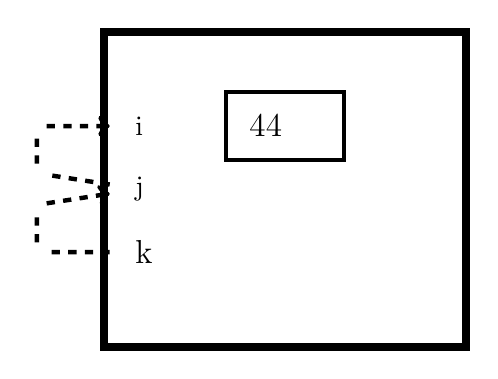
\begin{tikzpicture}
    \node[draw,text width=4cm,minimum height=4cm,minimum width=2cm, line width=0.1cm, inner sep=0.3cm] (a) at (-4, 2) {};
    \node[xshift=-8mm, yshift=8mm] (ji_arr) at (a.west) {};
    \node[xshift=-8mm, yshift=-8mm] (k_arr) at (a.west) {};
    \node[xshift=-8mm, yshift=2mm] (j_arr) at (a.west) {};
    \node[xshift=-8mm, yshift=-2mm] (kj_arr) at (a.west) {};

    \node[text width=1mm,minimum height=1mm,minimum width=1mm, line width=0.05cm, inner sep=0.3cm, xshift=5mm, yshift=8mm] (ival) at (a.west) {\normalsize{i}};
    \node[draw, text width=9mm,minimum height=1mm,minimum width=5mm, line width=0.05cm, inner sep=0.3cm, yshift=8mm] (ivalbox) at (a.center) {\large{44}};
    \node[text width=1mm,minimum height=1mm,minimum width=1mm, line width=0.05cm, inner sep=0.3cm, xshift=5mm] (jval) at (a.west) {\normalsize{j}};

    \node[text width=1mm,minimum height=1mm,minimum width=1mm, line width=0.05cm, inner sep=0.3cm, xshift=5mm, yshift=-8mm] (kval) at (a.west) {\large{k}};

   \draw [dashed, ultra thick, ->] (kval)[xshift=1mm] -- (k_arr) -- (kj_arr) -- (jval)[xshift=1mm];
   \draw [dashed, ultra thick, ->] (jval)[xshift=1mm] -- (j_arr) -- (ji_arr) -- (ival)[xshift=1mm];

\end{tikzpicture}
}
Here's the relevant rule: \EMPHASIZE{A reference can refer to another reference}. In other words, a reference variable can reference a variable or it can reference another reference variable.

\begin{ex}
What is the output?

\begin{consolethree}[escapeinside=||]
void f(int & a, double c)
{
    a = a + int(c);
    c = 1.0;
}

void g(int & b, double & c)
{
    b *= 2 + int(c);
    c = 0.0;
    f(b, c);
}

int main()
{
    int x = 42;
    double y = 3.14;
    g(x, y);
    std::cout << x << ' ' << y << std::endl;
    return 0;
}
\end{consolethree}

(Suggestion: Drawing a memory model might help.)
\end{ex}

Here's another rule: \EMPHASIZE{References must be initialized. Once you declare a reference, it must immediately refer to the memory of another variable}. Try this:

\begin{consolethree}[escapeinside=||]
int i = 5;
int & j; // create a reference variable ...
j = i;   // ... and *then* make the reference
\end{consolethree}

\begin{ex}
Does this work?

\begin{consolethree}[escapeinside=||]
int i = 5;
int & j = i + 1;
\end{consolethree}

Or this?

\begin{consolethree}[escapeinside=||]
int i = 5;
int k = 6;
int & j = i + k;
\end{consolethree}

Why?
\end{ex}

Yet another rule: \EMPHASIZE{Variable references must be initialized to variables or another reference (not an expression)} (This one is kind of obvious.) Here's an example:

\begin{ex}
Of course you know that you can do this:

\begin{consolethree}[escapeinside=||]
double x = 3.14;
int y = x;
\end{consolethree}

What about this:

\begin{consolethree}[escapeinside=||]
double x = 3.14;
int & y = x;
\end{consolethree}
\end{ex}

Rules, rules, rules ... \EMPHASIZE{The type of a reference must match the type it's referring to}.

\begin{ex}
What is the output? (Or find the errors).

\begin{consolethree}[escapeinside=||]
void swap(int & b, int & c)
{
    int t = b;
    b = c;
    c = t;
}

int main()
{
    int x = 42;
    double y = 1.234;
    swap(x, y);
    std::cout << x << ' ' << y << std::endl;
    return 0;
}
\end{consolethree}
\end{ex}

\begin{ex}
What is the output? (Or is there an error?)

\begin{consolethree}[escapeinside=||]
void g(double & b, double & c)
{
    b *= 2 + int(c);
    c = 0.0;
}

int main()
{
    int x = 42;
    double y = 3.14;
    g(x, y);
    std::cout << x << ' ' << y << std::endl;
    return 0;
}
\end{consolethree}

(Suggestion: Drawing a memory model might help.)
\end{ex}

\begin{ex}
You now know this works:

\begin{consolethree}[escapeinside=||]
int i = 0;
int & a = i;
\end{consolethree}

What about the following?

\begin{consolethree}[escapeinside=||]
int i = 0;
const int & a = i;
\end{consolethree}

\begin{consolethree}[escapeinside=||]
const int i = 0;
const int & a = i;
\end{consolethree}

\begin{consolethree}[escapeinside=||]
const int i = 0;
int & a = i;
\end{consolethree}

Try all of them. Give a reason for those that does not work. For those that work, can you change the value of \texttt{i} using \texttt{i}?

\verb!i = 42;!

Can you change the value of \texttt{i} using \texttt{a}?

\verb!a = 42;!

Why?
\end{ex}

\begin{ex}
What is the output? (Or find all the errors).

\begin{consolethree}[escapeinside=||]
void g(const int & b, const double & c)
{
    b *= 2 + c;
    c = 0.0;
    f(b, c);
}

int main()
{
    const int x = 42;
    double y = 3.14;
    g(x, y);
    std::cout << x << ' ' << y << std::endl;
    return 0;
}
\end{consolethree}
\end{ex}

\begin{ex}
What is the output? (Or find all the errors).

\begin{consolethree}[escapeinside=||]
void g(int & b, const double & c)
{
    b *= 2 + c;
    c = 0.0;
    f(b, c);
}

int main()
{
    const int x = 42;
    double y = 3.14;
    g(x, y);
    std::cout << x << ' ' << y << std::endl;
    return 0;
}
\end{consolethree}
\end{ex}

As mentioned before, a variable reference must reference a variable (or another reference). One exception is that \EMPHASIZE{a constant reference can refer to a constant}. Try this:

\verb!const int & i = 5;!

On the other hand the following won't work since you
already know that a reference must refer to a variable:

\verb!int & i = 5;!

A \EMPHASIZE{constant reference} is a reference that refers to a value and
treat that value as a constant.

\begin{consolethree}[escapeinside=||]
int x = 42;
const int & y = x; // y is a const ref to x

const int a = 0;
const int & b = a; // b is a const ref to a
\end{consolethree}

It's very important to remember that if \texttt{x} is a non-constant variable and \texttt{y} is a constant reference to \texttt{x}, then you cannot change the value of \texttt{x} using \texttt{y} -- because \texttt{y} views the value of \texttt{x} as though it's constant. However \texttt{x} can still change it's value:

\begin{consolethree}[escapeinside=||]
int x = 42;
const int & y = x;
std::cout << x << ' ' << y << '\n'

x = 0; // changing x ... OK
std::cout << x << ' ' << y << '\n'

y = -1; // changing x using y ... BAD!!!
\end{consolethree}

\begin{ex}
What is the output? (Or find the error)

\begin{consolethree}[escapeinside=||]
#include <iostream>

int f(int x[], int & len)
{
    int p = 1;
    for (int i = 0; i < len; i++)
    {
        p *= x[i];
    }
    return p;
}

int main()
{
    int a[] = {1, 2, 3};
    std::cout << f(a, 3) << std::endl;
    return 0;
}
\end{consolethree}
\end{ex}

\begin{ex}
After declaring a reference can the reference change the variable it's referring to? Does = work?

\begin{consolethree}[escapeinside=||]
int x = 1;
int y = 2;
int & z = x; // make z refer to x
z = 0;
std::cout << x << ' ' << y << ' ' << z << std::endl;

z = y; // make z refer to y ... can we?
z = -1;
std::cout << x << ' ' << y << ' ' << z << std::endl;
\end{consolethree}
\end{ex}

Here the rule: \EMPHASIZE{a reference variable cannot refer to another variable after it's initialization.}


\newpage\EMPHASIZE{Return value or pass-by-reference???}

Now we have a dilemma ...

The following is a simple \texttt{square()} function:

\begin{consolethree}[escapeinside=||]
double square(double x)
{
    return x * x;
}

int main()
{
    std::cout << square(3.14) << std::endl;
    return 0;
}
\end{consolethree}

But you know that you can also do this:

\begin{consolethree}[escapeinside=||]
void square(double x, double & theSquare)
{
    theSquare = x * x;
}

int main()
{
    double theSquare = 0.0;
    square(3.14, theSquare);
    std::cout << theSquare << std::endl;
    return 0;
}
\end{consolethree}

Make sure you run it.

Which should you use??? (Don't you hate making decisions ...)

In general, if your function is like a mathematical function that computes a value, then you should use a return value. (Principle of least surprise.)

For instance look at the above example. Notice how clumsy is the usage of the \texttt{square()} function.

If you have a function that computes two values, then you might want to have to have two pass-by-reference variables. Of course you can have two different functions. Here's an example:

Here's functions:

\begin{consolethree}[escapeinside=||]
double max(int x[], int len)
{
    double m = x[0];
    for (int i = 1; i < len; i++)
    {
        if (m < x[i]) m = x[i];
    }
    return m;
}

double min(int x[], int len)
{
    double m = x[0];
    for (int i = 1; i < len; i++)
    {
        if (m > x[i]) m = x[i];
    }
    return m;
}
\end{consolethree}

You can combine them into one:

\begin{consolethree}[escapeinside=||]
void max_min(int x[], int len,
             int & max, int & min)
{
    double max = x[0];
    double min = x[0];
    for (int i = 1; i < len; i++)
    {
        if (max < x[i]) max = x[i];
        if (min > x[i]) min = x[i];
    }
}
\end{consolethree}

If your program(s) always have to compute both the maximum and minimum, then the second version might be more useful. In fact it's faster than calling both \texttt{max()} and \texttt{min()} which requires \EMPHASIZE{two} function calls and also \EMPHASIZE{two} scans of the array.

However this means that one fine day, if you really need to compute only the minimum of an array, you have to call this function and you have to create a dummy variable for the max which is not going to be used:

\begin{consolethree}[escapeinside=||]
double x, y;
max_min(a, 10, x, y); // a is some array of length 10
... only x is used ...
\end{consolethree}

Or you have to write a \texttt{min()} function.

A basic principle of good software design is to design each function to perform one task and not two.

Now if you look at our \texttt{swap()} function

\begin{consolethree}[escapeinside=||]
void swap(int & a, int & b)
{
    int t = a;
    a = b;
    b = t;
}
\end{consolethree}

It does not perform a numerical computation; there is really no return value. It performs a transformation on variables. That's why the design of this function is reasonable.


\newpage\EMPHASIZE{Prototypes for references}

How do you write function prototypes for pass-by-reference parameters?

Easy! It's the same as your other variables. For instance if you have this function:

\begin{consolethree}[escapeinside=||]
void f(int a, double & b, char & c, const bool & b)
{
    ... code ...
}
\end{consolethree}

The function prototype is just

\verb!void f(int, double &, char &, const bool &);!

That's all there is to it. So there's
nothing new here.

\begin{ex}
Given this code

\begin{consolethree}[escapeinside=||]
#include <iostream>

int f(int & a, double & b)
{
    a++;
    b += a;
    return a * b
}

int main()
{
    int x = 42;
    double y = 1;
    int z = f(x, y);
    std::cout << x << ' ' << y << ' ' << z
              << std::endl;
    return 0;
}
\end{consolethree}

Rewrite it into this form:

\begin{consolethree}[escapeinside=||]
#include <iostream>

// prototype of f() here

int main()
{
    int x = 42;
    double y = 1;
    int z = f(x, y);
    std::cout << x << ' ' << y << ' ' << z
              << std::endl;
    return 0;
}

int f(int & a, double & b)
{
    a++;
    b += a;
    return a * b
}
\end{consolethree}

Run your program to make sure that you did it correctly.
\end{ex}

\begin{ex}
Here's the \texttt{swap()} example again.

\begin{consolethree}[escapeinside=||]
void swap(int & b, int & c)
{
    int t = b;
    b = c;
    c = t;
}

int main()
{
    int x = 42;
    int y = 1;
    swap(x, y);
    std::cout << x << ' ' << y << std::endl;
    return 0;
}
\end{consolethree}

Write a header file for the \texttt{swap()} function. Implement the body of the \texttt{swap()} function in a separate source file. Test your program.
\end{ex}

\begin{ex}
One of the parameters in \texttt{f()} need not be a reference.

Which one?

\begin{consolethree}[escapeinside=||]
int f(int & a, double & b)
{
    b += a;
    return a * b
}
\end{consolethree}
\end{ex}
